% Options for packages loaded elsewhere
\PassOptionsToPackage{unicode}{hyperref}
\PassOptionsToPackage{hyphens}{url}
%
\documentclass[
]{article}
\usepackage{lmodern}
\usepackage{amssymb,amsmath}
\usepackage{ifxetex,ifluatex}
\ifnum 0\ifxetex 1\fi\ifluatex 1\fi=0 % if pdftex
  \usepackage[T1]{fontenc}
  \usepackage[utf8]{inputenc}
  \usepackage{textcomp} % provide euro and other symbols
\else % if luatex or xetex
  \usepackage{unicode-math}
  \defaultfontfeatures{Scale=MatchLowercase}
  \defaultfontfeatures[\rmfamily]{Ligatures=TeX,Scale=1}
\fi
% Use upquote if available, for straight quotes in verbatim environments
\IfFileExists{upquote.sty}{\usepackage{upquote}}{}
\IfFileExists{microtype.sty}{% use microtype if available
  \usepackage[]{microtype}
  \UseMicrotypeSet[protrusion]{basicmath} % disable protrusion for tt fonts
}{}
\makeatletter
\@ifundefined{KOMAClassName}{% if non-KOMA class
  \IfFileExists{parskip.sty}{%
    \usepackage{parskip}
  }{% else
    \setlength{\parindent}{0pt}
    \setlength{\parskip}{6pt plus 2pt minus 1pt}}
}{% if KOMA class
  \KOMAoptions{parskip=half}}
\makeatother
\usepackage{xcolor}
\IfFileExists{xurl.sty}{\usepackage{xurl}}{} % add URL line breaks if available
\IfFileExists{bookmark.sty}{\usepackage{bookmark}}{\usepackage{hyperref}}
\hypersetup{
  pdfauthor={Rockefeller University, The Vertebrate Genome Lab},
  hidelinks,
  pdfcreator={LaTeX via pandoc}}
\urlstyle{same} % disable monospaced font for URLs
\usepackage[margin=1in]{geometry}
\usepackage{graphicx,grffile}
\makeatletter
\def\maxwidth{\ifdim\Gin@nat@width>\linewidth\linewidth\else\Gin@nat@width\fi}
\def\maxheight{\ifdim\Gin@nat@height>\textheight\textheight\else\Gin@nat@height\fi}
\makeatother
% Scale images if necessary, so that they will not overflow the page
% margins by default, and it is still possible to overwrite the defaults
% using explicit options in \includegraphics[width, height, ...]{}
\setkeys{Gin}{width=\maxwidth,height=\maxheight,keepaspectratio}
% Set default figure placement to htbp
\makeatletter
\def\fps@figure{htbp}
\makeatother
\setlength{\emergencystretch}{3em} % prevent overfull lines
\providecommand{\tightlist}{%
  \setlength{\itemsep}{0pt}\setlength{\parskip}{0pt}}
\setcounter{secnumdepth}{-\maxdimen} % remove section numbering

\title{RU Genome Assembly, Session 1}
\author{Rockefeller University, The Vertebrate Genome Lab}
\date{}

\begin{document}
\maketitle

{
\setcounter{tocdepth}{2}
\tableofcontents
}
\hypertarget{an-introduction-to-genome-assembly}{%
\section{An introduction to genome
assembly}\label{an-introduction-to-genome-assembly}}

\hypertarget{principles-and-practicalities-of-assembling-evaluating-and-using-a-reference-genome}{%
\paragraph{Principles and practicalities of assembling, evaluating and
using a reference
genome}\label{principles-and-practicalities-of-assembling-evaluating-and-using-a-reference-genome}}

\leavevmode\hypertarget{hello}{}%
Giulio Formenti, Ph.D.\\
Laboratory of Neurogenetics of Language\\
Vertebrate Genome Laboratory\\
The Rockefeller University\\
\href{mailto:gformenti@rockefeller.edu}{\nolinkurl{gformenti@rockefeller.edu}}

\textbf{In collaboration with the Vertebrate Genomes Laboratory}

\emph{March 22nd \& 25th - Monday \& Thursday}


\includegraphics[width=0.3\textwidth,height=\textheight]{../imgs/VGL_logo.png}

\includegraphics[width=0.15\textwidth,height=\textheight]{../imgs/RU_logo.png}

\hypertarget{overview}{%
\subsection{Overview}\label{overview}}

\begin{itemize}
\tightlist
\item
  \href{https://docs.conda.io/projects/conda/en/latest/user-guide/getting-started.html}{Introduction
  to Conda}
\item
  \href{https://snakemake.readthedocs.io/en/stable/}{Introduction to
  Snakemake}
\end{itemize}

\hypertarget{materials}{%
\subsection{Materials}\label{materials}}

\begin{itemize}
\tightlist
\item
  \href{https://git.imp.fu-berlin.de/cmazzoni/genome_evaluation_snakemake}{GEP
  - Genome evaluation pipeline}
\item
  Path on RU HPC to test data: /fakepath/to/data
\end{itemize}

\hypertarget{the-vertebrate-genomes-project}{%
\subsection{The Vertebrate Genomes
Project}\label{the-vertebrate-genomes-project}}

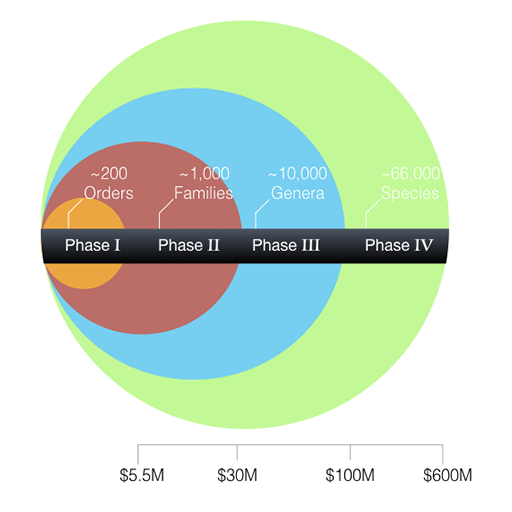
\includegraphics[width=0.3\textwidth,height=\textheight]{../imgs/VGP_phases.png}
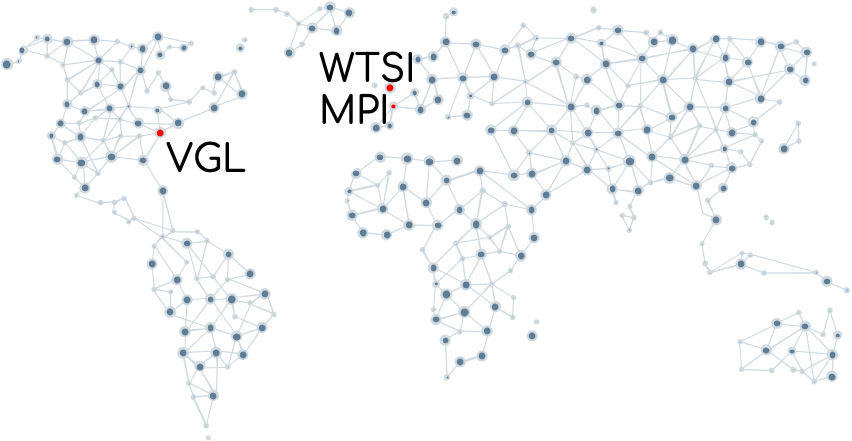
\includegraphics[width=0.6\textwidth,height=\textheight]{../imgs/VGP_map.png}

\href{https://vertebrategenomesproject.org/}{VGP website}\\

\includegraphics[width=0.3\textwidth,height=\textheight]{../imgs/VGP_logo.png}

\hypertarget{main-international-endeavours}{%
\subsection{Main international
endeavours}\label{main-international-endeavours}}

\begin{figure}
\centering

\includegraphics[width=0.3\textwidth,height=\textheight]{../imgs/B10K_logo.png}
\caption{B10K logo}
\end{figure}

\begin{figure}
\centering

\includegraphics[width=0.3\textwidth,height=\textheight]{../imgs/dToL_logo.png}
\caption{dToL logo}
\end{figure}


\includegraphics[width=0.3\textwidth,height=\textheight]{../imgs/GIGA_logo.jpg}

\includegraphics[width=0.3\textwidth,height=\textheight]{../imgs/EBP_logo.jpg}

\hypertarget{why-sequencing-the-dna}{%
\subsection{Why sequencing the DNA}\label{why-sequencing-the-dna}}

\emph{«A knowledge of sequences could contribute much\\
to our understanding of living matter»}

Frederick Sanger, 1980

\begin{figure}
\centering
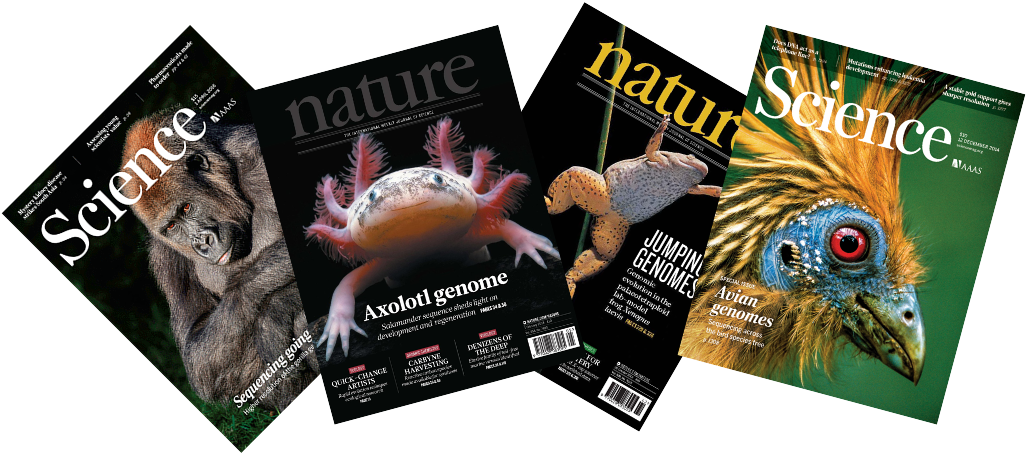
\includegraphics[width=0.7\textwidth,height=\textheight]{../imgs/science.png}
\caption{Science}
\end{figure}

\end{document}
